\section{Komunikační řetězec, vrstvový model datového přenosu, základní operace při zpracování signálu u digitálního komunikačního systému. Úrovně signálu a vztažné hodnoty, absolutní a relativní úroveň, útlum, zisk, odstup signálu od šumu, výkonová spektrální hustota, přenosová kapacita kanálu.
}

\subsection{Komunikační řetězec}

\begin{figure}[h]
    \centering
	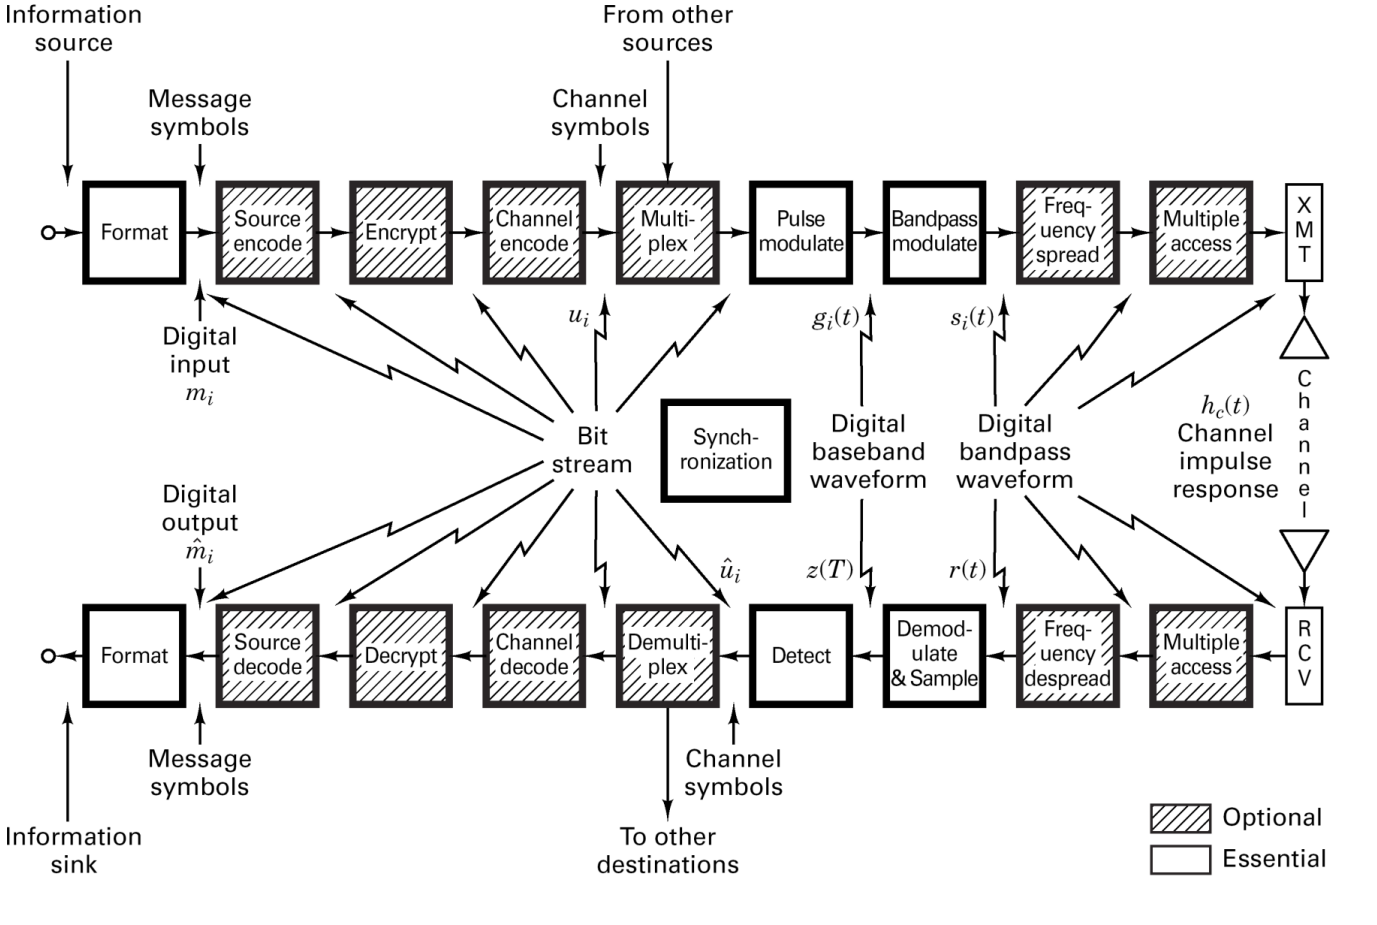
\includegraphics[width=0.9\textwidth]{images/01-kom-retezec.png}
    \caption{Komunikační řetězec}
    \label{komStr}
\end{figure}

\subsection{Základní operace}

\textbf{Format -- digitalizace signálu}: vzorkování, lineární a nelineární kvantování, pulzně kódová modulace.
\newline\textbf{Source encode -- zdrojové kódování}: kódování řeči, hudby a obrazu pro odstranění redundance, ztrátové (JPEG, MPEG) a bezeztrátové (Huffman) kódování.
\newline\textbf{Encrypt -- šifrování}: zabezpečení dat proti zneužití, symetrické a asymetrické systémy.
\newline\textbf{Channel encode -- kanálové kódování}: zabezpečení dat proti chybám (detekční nebo opravné kódy).
\newline\textbf{Multiplex}: sloučení více datových toků od více uživatelů do jednoho.
\newline\textbf{Pulse modulate -- tvarování pulzů}: tvarování pulsů za účelem snížení šířky pásma a potlačení mezisymbolových interferencí
\newline\textbf{Bandpass modulate -- modulace}: převod signálu ze základního pásma do přenosového. Různé modulace (MQAM, MPSK, MFSK, GMSK, ...).
\newline\textbf{Frequency spread -- kmitočtové rozprostření}: rozšíření kmitočtového spektra pro širokopásmové přenosy (eliminace úniků).
\newline\textbf{Multiple access -- mnohonásobný přístup}: metody přístupu -- časové (TDMA), kmitočtové (FDMA), kódové (CDMA), prostorové (SDMA), polarizační (PDMA).
\newline\textbf{XMT -- vysílač}
\newline\textbf{Synchronization -- synchronizace}: slouží pro zajištění přenosu, získání informace o časování symbolů, kmitočtu a fázi nosné vlny, časování rámců a další.
\newline\textbf{Channel -- přenosový kanál}: rušivé vlivy -- zpoždění rušení a další.
\newline\textbf{RCV -- přijímač}
\newline\textbf{Demodulate \& Sample -- demudulace a vzorkování}: převod signálu demodulátorem do základního pásma, ekvalizace a vzorkování ve vhodných okamžicích daných synchronizací.
\newline\textbf{Detect -- vyhodnocení symbolů}: detekce symbolů v závislosti na typu modulace.

\subsection{Úroveň signálu a vztažné hodnoty}
\textbf{Relativní úrovně} -- vztažné k úrovni ve vztažném místě 0. $P_0$ a $U_0$ je vztažný výkon respektive vztažné napětí ve vztažném bodě 0.
\[L_r=10*\log\frac{P_x}{P_0} \quad [dBr; W, W]\]
\[L_{ru}=20*\log\frac{U_x}{U_0} \quad [dBru; V, V]\]

\textbf{Absolutní úrovně} jsou vztažné k referenční hodnotě, tj. že za vztažné hodnoty se dosazuje referenční hodnota (např. $P_0 = 0,001$ Mw). Z je označení impedance.
\[L_m = 10*\log\frac{P}{P_0} = 10*\log\frac{\frac{U^2}{Z}}{\frac{P^2_0}{Z_0}} = 20*\log\frac{U}{U_0} + 10*\log\frac{Z}{Z_0} = L_u + \Delta Z\]

\textbf{Útlum (A)} se vypočítá jako $A = L_{m1} - L_{m2}$.
\newline\textbf{Zisk (G)} také označován jako \textbf{S} je opakem útlumu.
\newline\textbf{SNR -- odstup signál šum} -- je podíl výkonu signálu (S) k výkonu šumu (N)\[SNR = \frac{S}{N}\] nebo \[SNR = 10*\log_{10}\frac{S}{N} = 20*\log_{10}\frac{U_s}{U_n} \quad [dB, W, W, V, V]\]

\textbf{PSD -- výkonová spektrální hustota} udává rozložení výkonu při přenosu signálů s náhodným charakterem -- spojité kmitočtové spektrum. \[PSD = \frac{P}{B} \quad [W/Hz, W, Hz]\] kde B je šířka pásma.

\textbf{Přenosová kapacita kanálu} -- Maximální rychlost přenosu se nazývá kapacita kanálu (C). To je množství informace které lze přenést za jednotku času. Shannon-Hartley teorém
\[C = B*\log_2(1 + \frac{S}{N}) \quad [b/s, Hz, W, W]\]
\[C = 3,32B*\log_10(1 + \frac{S}{N})\]
\[C = \int\limits_B{\log_2\left[1 + \frac{S(f)}{N(f)}\right]df}\]

\clearpage
\section{Princip zvyšování odolnosti přenášené zprávy proti chybám, informační poměr kódu, Hammingova vzdálenost, podmínky možnosti detekce a korekce chyb.}

\clearpage
\section{Vlastnosti ovlivňující návrh protichybového kódového systému. ARQ systémy.}

\clearpage
\section{Rozdělení protichybových kódů. Schéma realizace procesu kódování blokových kódů a stromových kódů. RM kódy, jejich základní parametry. Obecné blokové schéma kodéru turbokódu, význam jeho částí, dekódování turbokódů. Přehled možností používaných pro zabezpečení proti dlouhým shlukům chyb.}

\clearpage
\section{Kryptografické metody zabezpečení datových přenosů, architektura bezpečnosti, služby bezpečnosti, mechanizmy bezpečnosti.}

\clearpage
\section{Telekomunikační síť, struktura, způsoby komunikace, přenosové prostředky.}

\clearpage
\section{Metalická vedení, náhradní schéma homogenního vedení, primární parametry, sekundární parametry jednotky a vzájemné vztahy. Konstrukce symetrických kabelových vedení používaných v přístupové síti, DM a x čtyřky. Modely elektrických parametrů kabelových vedení určené pro simulaci DSL.}

\clearpage
\section{DSL systémy, vlastnosti, referenční konfigurace, typické uspořádání přípojky, možnosti využití. Základní charakteristiky jednotlivých systémů xDSL, IDSL, HDSL, SDSL, ADSL, VDSL, vlastnosti, možnosti použití. DSL použité kódy a modulace, 2B1Q, QAM, TCM,DMT, CAP.}

\clearpage
\section{Vliv rušení na provoz xDSL, kategorizace, dosažitelná přenosová rychlost, model přeslechů (NEXT, FEXT), princip výpočtu přeslechů. Spektrální vlastnosti DSL přenosových systémů, správa spektra, cíle, metody.}

\clearpage
\section{PLC systémy, princip, základní parametry, použité modulace, vazební členy, začlenění do sítě.}
